\section{Paradigma \emph{Greedy}}

\subsection{Introduzione}

Il problema del memorylessness del paradigma \emph{Divide and Conquer} è stato risolto utilizzando il paradigma del \emph{Dynamic Programming}. Risolvendo un problema con la programmazione dinamica, però, la soluzione viene costruita componendo le soluzioni di sottoistanze, scegliendo di volta in volta la sottosoluzione migliore. Questa scelta può avvenire solo dopo aver calcolato \emph{tutte} le soluzioni alle sottoistanze.

Il paradigma \emph{Greedy} seleziona ad ogni iterazione la scelta più promettente, e calcola la soluzione alla sottoistanza relativa \emph{solo} a quella scelta.

Occorre dimostrare che la scelta non comprometta l'ottimalità della soluzione.

\subsection{Definizione}

Il paradigma \emph{Greedy} agisce in tre passi:
\begin{enumerate}
    \item Scelta \emph{Greedy}: compie una scelta che sembra essere quella più promettente, localmente ottima, che non comprometta la soluzione: la soluzione ottima conterrà quella scelta.
    \item \emph{Clean up}: l'istanza viene ripulita, in accordo con la scelta effettuata.
    \item \emph{Tail recursion}: viene risolta l'\emph{unica} istanza generata, come ultimo comando della funzione. Questo tipo di ricorsione può sempre essere scritto in maniera iterativa.
\end{enumerate}

Vanno quindi dimostrate due proprietà:
\begin{enumerate}
    \item la scelta \emph{Greedy} (SG) non compromette l'ottimalità della soluzione locale: \\
        $\exists S^*$ che contiene la scelta \emph{Greedy}
    \item $\exists S^*$ che, oltre alla scelta \emph{Greedy}, contiene la soluzione della sottoistanza ottenuta dal \emph{clean up}, detta sottoistanza residua
\end{enumerate}

\section{Selezione di attività}

\subsection{Definizione del problema}

Un problema che si presta ad essere risolto con il paradigma \emph{Greedy} è la selezione di attività. Data una risorsa condivisa e un insieme di attività che la utilizzano, come si può selezionare il massimo numero di attività compatibili? Formalmente si definiscono:
\begin{itemize}
    \item[--] Risorsa condivisa
    \item[--] Insieme di attività $S = \left\{ a_1, \cdots, a_n \right\}$ con $a_i = [s_i, f_i)$
    \item[--] Attività compatibili: $a_i$ è compatibile con $a_j$ se
        $[s_i, f_i) \cap [s_j, f_j) = \emptyset$
        o
        $(f_i \leq s_j ) \vee (f_j \leq s_i)$
\end{itemize}
L'obiettivo è determinare il sottoinsieme $S^* \subseteq S$ di attività mutualmente compatibili (intervalli a coppie disgiunti) di cardinalità massima.

\subsection{Soluzione \emph{Greedy}}

Senza perdita di generalità, si può assumere che le attività siano ordinate per tempo di fine non decrescente:
$f_1 \leq f_2 \leq \cdots \leq f_n$

L'intuizione è di selezionare di volta in volta l'istanza che finisce prima, in modo da lasciare il più tempo possibile \emph{compatto} per selezionare le altre. Nella fase di \emph{clean-up}, si scorrono le attività in ordine, eliminando quelle non compatibili. È sufficiente fermarsi alla prima istanza compatibile che si trova: successive istanze che non sono compatibili con quella selezionata, non saranno compatibili neppure con quella trovata per prima, e saranno eliminate successivamente.

\begin{algorithm}[H]
\caption{Selezione di attività, implementazione ricorsiva}\label{alg:asrec}
\begin{algorithmic}[1]
    \Procedure{REC\_AS}{$\vec{s}, \vec{f}, g$}
        \State $n \gets \vec{s}.len$
        \If{$g > n$}
        \Comment{Problema vuoto}
            \State return
        \EndIf
        \State $SG \gets \left\{ a_g \right\}$
        \Comment{Prima attività, scelta \emph{Greedy}}
        \State $i \gets g+1$
        \While{ $\left( s_i < f_g \right) \wedge \left( i \leq n \right)$}
            \State $i \gets i+1$
            \Comment{\emph{Clean-up}}
        \EndWhile
        \State return $SG \cup \Call{REC\_AS}{\vec{s}, \vec{f}, i}$
        \Comment{\emph{Tail recursion}}
    \EndProcedure
\end{algorithmic}
\end{algorithm}

\begin{algorithm}[H]
\caption{Selezione di attività, implementazione iterativa}\label{alg:asiter}
\begin{algorithmic}[1]
    \Procedure{GREEDY\_AS}{$\vec{s}, \vec{f}$}
        \State $n \gets \vec{s}.len$
        \State $g \gets 1$
        \State $A \gets \left\{ a_g \right\}$
        \Comment{Insieme di attività scelte $A$}
        \For{$i \gets 2 $ to $ n $ }
        \Comment{Alterna selezione e \emph{clean-up}}
            \If{$ s_i \geq f_g $}
                \State $g \gets i$
                \State return $A \cup \left\{ a_g \right\}$
            \EndIf
        \EndFor
        \State return $A$
    \EndProcedure
\end{algorithmic}
\end{algorithm}

\subsection{Dimostrazione della correttezza}

\subsubsection{Proprietà di scelta \emph{Greedy}}

Occorre dimostrare che esiste una soluzione ottima $A^*$ che contiene la scelta \emph{Greedy} ${a_1}$. Si procede per \emph{cut and paste}: Sia $\hat{A}$ una soluzione ottima. Se ${a_1} \in \hat{A}$ si conclude, se no si sostituisce un'attività in $\hat{A}$ con la scelta \emph{Greedy} e si dimostra che l'insieme ottenuto è ancora ottimo e contiene la scelta \emph{Greedy}.
Sia $\hat{i} =  \argmin\limits_i \{ a_i \in \hat{A} \} $, e sia
\[
A^* = \hat{A} 
\;
\underbracket[1pt]{
\setminus \left\{ a_{\hat{i}} \right\} 
}_{\text{\emph{cut}}}
\;
\underbracket[1pt]{
\vphantom{ \setminus \left\{ a_{\hat{i}} \right\} }
\cup \left\{ a_1 \right\}
}_{\text{\emph{paste}}}
\]

Va dimostrato che $a_1$ è compatibile con ogni $a_j$, ossia 
$\forall a_j \in \hat{A} \setminus \left\{ a_{\hat{i}} \right\} \Rightarrow f_1 \leq s_j$
\\
Vale $f_1 \leq f_{\hat{i}}$ perché $a_1$ è la scelta \emph{Greedy}, e $f_{\hat{i}} \leq s_j$ perché $\hat{A}$ contiene attività compatibili, per cui $f_1 \leq s_j$, e $A^*$ è ammissibile. Inoltre $|A^*| = |\hat{A}|$, quindi è anche soluzione ottima. Per costruzione $A^*$ contiene la scelta \emph{Greedy}, e si conclude.

\subsubsection{Proprietà di sottostruttura ottima}

Va dimostrata l'esistenza di una soluzione ottima $A^*$ che, oltre ad $a_1$, contiene una soluzione ottima al sottoproblema residuo $S_r$. 
Il sottoproblema residuo si ottiene effettuando il \emph{clean-up}, eliminando tutte le attività $a_j$, con $j>1$, per cui $s_j < t_1$, fermandosi o per $g : f_1 \leq s_g$, o quando tutte le attività sono state eliminate. $S_r$ è quindi un suffisso di attività che parte da $g$.

Si possono verificare due casi:

$S_r = \emptyset $: tutte le attività sono in conflitto con $a_1 \Rightarrow A^*=\left\{ a_1 \right\}$
e la soluzione al $S_r$ è $sol( A^* \setminus \left\{ a_1 \right\} ) = sol ( \emptyset ) = \emptyset$.
La soluzione al $S_r$ è vuota, e $A^*$ oltre alla scelta \emph{Greedy} non contiene nulla.

$S_r = \left\{ a_g, a_{g+1}, \cdots, a_n \right\}, g>1$: almeno un'attività è compatibile con $a_1$, la soluzione ottima dovrà contenere almeno due attività. Si deve dimostrare che $A^* \setminus \left\{ a_1 \right\}$ è soluzione ammissibile e ottima per $S_r$.

Per dimostrare l'ammissibilità vanno mostrate due proprietà: le attività in $A^* \setminus \left\{ a_1 \right\}$ devono essere mutualmente compatibili, e lo sono perché questo è un sottoinsieme di attività compatibili; $A^* \setminus \left\{ a_1 \right\} \subseteq S_r$, devono essere attività contenute in $S_r$, e lo sono, perché $S_r$ è stato ottenuto proprio eliminando $a_1$ e tutte le attività non compatibili con questa, ossia $a_2, \cdots, a_{g-1}$, e nessuna delle attività eliminate per ottenere $S_r$ potrebbe convivere con $a_1$.

Per dimostrare l'ottimalità di $A^* \setminus \left\{ a_1 \right\}$ per $S_r$ si procede per assurdo, supponendo che $A^* \setminus \left\{ a_1 \right\}$ \emph{non} sia ottima per $S_r$. Deve quindi esistere un sottoinsieme $\hat{A} \subseteq S_r$ di attività compatibili
contenente $a_g$, la scelta \emph{Greedy} per $S_r$,
con $|\hat{A}| > |A^*|-1$, e se questo fosse vero si troverebbe una soluzione a $S$ migliore di $A^*$, che era ottima.
Si può aggiungere a questo insieme $a_1$ che di sicuro non è già presente, non essendo in $S_r$, ottenendo $|\hat{A} \cup \left\{ a_1 \right\} | > |A^*|$. 
Tutte le attività in $\hat{A}$ sono compatibili con $a_1$, infatti $f_1 < s_g$ per costruzione del problema residuo, $s_g < f_g$ per ogni attività e $f_g < s_i$ per ogni attività in $\hat{A}$, per la compatibilità di $a_g$.
Questo conduce ad un assurdo, perché $A^*$ era la soluzione ottima.

\section{Compressione di un file}

\subsection{Definizione del problema}

Un file può essere visto come stringa di caratteri di un alfabeto, $F \in \Sigma^*$. A ciascun carattere è associata una frequenza: $\forall c \in \Sigma : f(c) \in [0,1]$. Il file usa solo un sottoalfabeto $C \subseteq \Sigma : c \in C \Rightarrow f(c) > 0$.

La compressione è una mappa che associa ad ogni carattere una stringa di bit:
\[
    % l_F : \Sigma \rightarrow \left\{ 0,1 \right\}^* \\
    e : C \rightarrow \left\{ 0,1 \right\}^*
\]

Le $e(c)$ sono dette parole di codice, o \emph{codeword}.
Le mappe di codifica sono memorizzate in una struttura detta \emph{trie}, un albero binario etichettato.
Per ricostruire il file originale, è sufficiente mantenere due puntatori, uno sul trie e uno sul file codificato, scorrendo il file e scendendo l'albero, tornando alla radice ogni volta che si arriva ad una foglia.

Un esempio di file, codificato con caratteri ASCII a 8 bit, è caratterizzato dalle frequenze dei caratteri che compaiono nel file:
\begin{equation*}
    \begin{array}[H]{rcccccc}
        \texttt{C:} & a & b & c & d & e & f \\
        \texttt{freq rel:} & 0.45 & 0.13 & 0.12 & 0.16 & 0.09 & 0.05
    \end{array}
\end{equation*}
Se $|F| = 100M$ caratteri, per memorizzarlo senza compressione sono necessari $800 Mbit$. Il file usa solo 6 dei 256 caratteri possibili, sono quindi sufficienti meno bit per memorizzarli. In generale, per memorizzare $k$ caratteri sono necessari $\left\lceil \log_2 k \right\rceil$ bit. In questo caso, 3 bit sono sufficienti, e il file si può quindi memorizzare con $300 Mbit$ utilizzando una codifica a lunghezza costante (\emph{fixed-length encoding}).
\begin{equation*}
    \begin{array}[H]{rcccccc}
        \texttt{C:} & a & b & c & d & e & f \\
        \texttt{codifica:} & 000 & 001 & 010 & 011 & 100 & 101
    \end{array}
\end{equation*}
Oltre al file compresso occorre memorizzare anche la mappa di codifica, ma la sua dimensione è generalmente irrisoria rispetto a quella del file.
In \rfig{tree:lungcost} è mostrato il \emph{trie} della codifica a lunghezza costante.
\begin{figure}[h]
\begin{center}
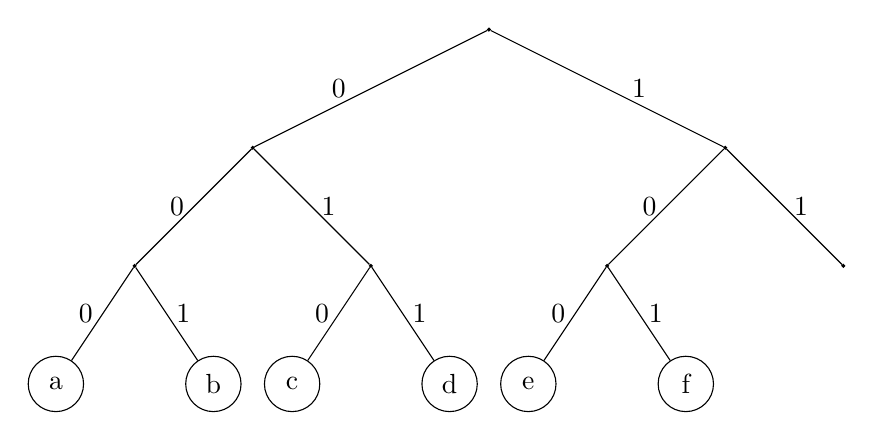
\begin{tikzpicture}[
        level/.style={sibling distance=60mm/#1},
        redge/.style={right,draw=none},
        ledge/.style={left,draw=none},
        inner/.style={draw,circle,fill=black,inner sep=0pt,minimum width=0pt},
        % inner/.style={inner sep=0pt,minimum width=0pt},
        % inner/.style={inner sep=0pt,minimum width=-1pt},
        leaf/.style={circle,draw,minimum width=20pt},
        ]
    \node (z) [inner] {}
    child {
        node [inner] (a) {}
        child {
            node [inner] (b) {}
                child {
                    node [leaf] (b1) {a}
                    edge from parent node[ledge] {0}
                }
                child {
                    node [leaf] (b2) {b}
                    edge from parent node[redge] {1}
                }
            edge from parent node[ledge] {0}
        }
        child {
            node [inner] (e) {}
                child {
                    node [leaf] (e2) {c}
                    edge from parent node[ledge] {0}
                }
                child {
                    node [leaf] (e2) {d}
                    edge from parent node[redge] {1}
                }
            edge from parent node[redge] {1}
        }
        edge from parent node[ledge] {0$\;\;$} % edge da (a)
    }
    child {
        node [inner] (c) {}
        child {
            node [inner] (d) {}
                child {
                    node [leaf] (d1) {e}
                    edge from parent node[ledge] {0}
                }
                child {
                    node [leaf] (d2) {f}
                    edge from parent node[redge] {1}
                }
            edge from parent node[ledge] {0}
        }
        child {
            node [inner] (c2) {}
            edge from parent node[redge] {1}
        }
        edge from parent node[redge] {$\;\;$1}
    }
    ; % end of the node
\end{tikzpicture}
\end{center}
\caption{\emph{Trie} della codifica a lunghezza costante}
\label{tree:lungcost}
\end{figure}
Questo \emph{trie} è chiaramente non ottimo: una delle foglie non è utilizzata.
Assegnare ancora meno bit ad alcune lettere può condurre ad una compressione ancora maggiore, ma bisogna assicurarsi che la codifica risultante sia libera da prefissi (\emph{prefix code}). Per esempio la seguente codifica
\begin{equation*}
    \begin{array}[H]{rcccccc}
        \texttt{C:} & a & b & c & d & e & f \\
        \texttt{codifica:} & 0 & 00 & 01 & 1 & 10 & 11
    \end{array}
\end{equation*}
non permette di distinguere $e(`ad \textit{'})$ e $e(`c \textit{'})$.
Questa codifica però fornisce il limite inferiore alla grandezza possibile del file compresso:
\begin{equation*}
    |F| \left( 0.45*1 + 0.13*2 + \dots \right) = 153M
\end{equation*}
Per assicurare la decodificabilità deve valere
\begin{equation*}
    \nexists \, c_1, c_2 : e(c_1) \text{ è prefisso di } e(c_2)
\end{equation*}
Si definisce profondità di un carattere $c$ in un \emph{trie} la quantità $d_T(c) = |e(c)|$.
\\
Il costo di una codifica è
\begin{equation*}
    \sum_{c \in C}\left( |F| f(c) \right) d_T(c) = 
    |F| \sum_{c \in C} f(c) d_T(c) = 
    |F| B(T)
\end{equation*}
dove $B(T)$ è la somma della profondità delle foglie del \emph{trie} pesata con le frequenze del carattere.
\\
L'obiettivo è minimizzare $B(T)$ su tutti i possibili \emph{trie} per l'insieme di caratteri $C$.

\subsection{Soluzione \emph{Greedy}}

Si è quindi definito un problema di ottimizzazione molto chiaro: va determinato 
\begin{equation*}
    T^* = \argmin \left\{ B(T) : T \right\}
\end{equation*}

\subsection{Dimostrazione della correttezza}

\subsubsection{Proprietà di scelta \emph{Greedy}}

\subsubsection{Proprietà di sottostruttura ottima}

\subsection{autocomplete}
Snippet di \LaTeX{} che tornano spesso utili

Una bella scatola:
\begin{equation}
    \boxed{x^2+y^2 = z^2}
\end{equation}

Numeri nei casi
\begin{numcases}{T(n)=}
    2^3 \label{escaso1} \\
    2^4 \label{escaso2} 
\end{numcases}

Sotto numeri
\begin{subnumcases}{T(n)=}
    2^3 \label{escaso3} \\
    2^4 
\end{subnumcases}

Liste compatte
\begin{itemize}[noitemsep,topsep=0pt,parsep=0pt,partopsep=0pt]
    \item qualcosa
    \item[+] qualcosa
    \item[*] qualcosa
    \item[--] qualcosa
\end{itemize}

Parole in libertà per l'autocomplete: 
à
è
ì
ò
ù
perché
così
sì
può
più

Viva vim se scrivi \verb|<C-k>`e| o \verb|<C-k>e`| in insert mode mette una è

% delirio doppio di vim se scrivi \verb|<C-k>da| in insert mode mette ``Hiragana letter DA'' che purtroppo non posso mostrarvi %だ
% insomma i digraph sono tanti e belli

Spazietti fra equazioni
\begin{equation*}
    A^{[0]}(x) = \sum_{j=0}^{\frac{n}{2}-1} a_{2j}x^j
    \quad \text{ e } \quad
    A^{[1]}(x) = \sum_{j=0}^{\frac{n}{2}-1} a_{2j+1}x^j
\end{equation*}

Un gustoso algoritmo
\begin{algorithm}[H]
\caption{Divide and Conquer}\label{alg:dncmock}
\begin{algorithmic}[1]
    \Procedure{D\&C}{$i$}
        \If{$|i| \leq n_0$}                             \Comment{BASE}
            \State *risolvo direttamente*
        \EndIf
        \State $<i_1, i_2, \dots, i_k> \gets A_D(i)$    \Comment{DIVIDE}
        \For{$j \gets 1 $ to $ k $ }                    \Comment{RECURSE}
            \State $s_j \gets $ \Call{D\&C}{$i_j$}
        \EndFor
        \State $s \gets A_C(<s_1, s_2, \dots, s_k>)$    \Comment{CONQUER}
        \State return $s$
    \EndProcedure
\end{algorithmic}
\end{algorithm}

Un alberello
\begin{center}
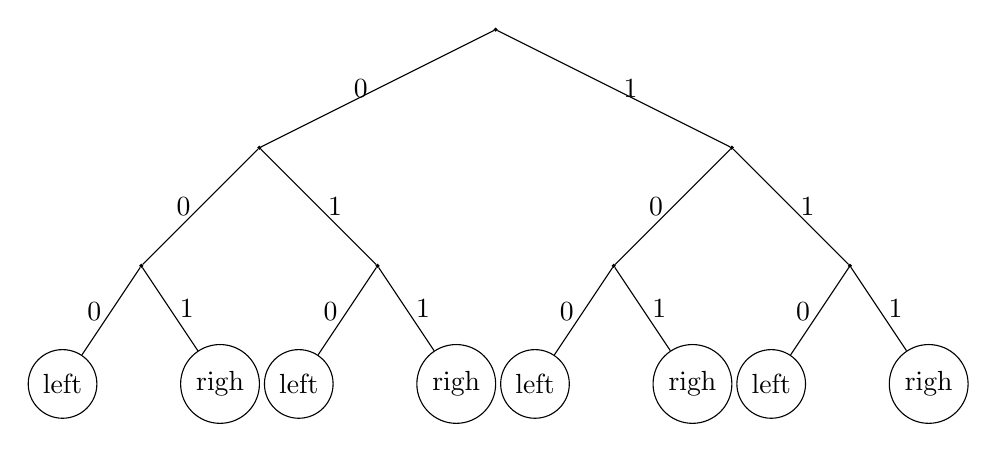
\begin{tikzpicture}[
        level/.style={sibling distance=60mm/#1},
        redge/.style={right,draw=none},
        ledge/.style={left,draw=none},
        inner/.style={draw,circle,fill=black,inner sep=0pt,minimum width=0pt},
        % inner/.style={inner sep=0pt,minimum width=0pt},
        % inner/.style={inner sep=0pt,minimum width=-1pt},
        leaf/.style={circle,draw},
        ]
    \node (z) [inner] {}
    child {
        node [inner] (a) {}
        child {
            node [inner] (b) {}
                child {
                    node [leaf] (b1) {left}
                    edge from parent node[ledge] {0}
                }
                child {
                    node [leaf] (b2) {righ}
                    edge from parent node[redge] {1}
                }
            edge from parent node[ledge] {0}
        }
        child {
            node [inner] (e) {}
                child {
                    node [leaf] (e2) {left}
                    edge from parent node[ledge] {0}
                }
                child {
                    node [leaf] (e2) {righ}
                    edge from parent node[redge] {1}
                }
            edge from parent node[redge] {1}
        }
        edge from parent node[ledge] {0} % edge da (a)
    }
    child {
        node [inner] (c) {}
        child {
            node [inner] (d) {}
                child {
                    node [leaf] (d1) {left}
                    edge from parent node[ledge] {0}
                }
                child {
                    node [leaf] (d2) {righ}
                    edge from parent node[redge] {1}
                }
            edge from parent node[ledge] {0}
        }
        child {
            node [inner] (f) {}
                child {
                    node [leaf] (f1) {left}
                    edge from parent node[ledge] {0}
                }
                child {
                    node [leaf] (f2) {righ}
                    edge from parent node[redge] {1}
                }
            edge from parent node[redge] {1}
        }
        edge from parent node[redge] {1}
    }
  ; % end of the node
\end{tikzpicture}
\end{center}
